\documentclass[12pt,a4paper]{article}
\usepackage{graphicx}
\usepackage{sidecap}
\usepackage{subfigure}
\usepackage{wrapfig}
\usepackage{float}
\floatstyle{boxed} 
\restylefloat{figure}
\usepackage{caption}
\captionsetup[figure]{name=Fig.}
\usepackage[section]{placeins}
\usepackage{listings}
% Use \begin{lstlisting} or \lstinputlisting[language=Python]{source_filename.py}

% Title Page
\title{
	
\includegraphics[width=0.3\textwidth]{pictures/iitr-logo}\\~\\
	{\LARGE Breaking Diffie-Hellman protocol using Parameter Injection through Man~in~the~Middle (MITM) Attack}
}
\author{
	Jay Hitesh Bosamiya \& Rakholiya Jenish\\
	{\small 3\textsuperscript{rd} year, B. Tech. (CSE)}\\
	{\small Enr No: 13114024 \& 13114044}\\
	\\
	{\small jaybosamiya@acm.org \& rjeniuec@iitr.ac.in}\\
	\\
	Guided by\\
	Prof. Sandeep Kumar Garg
}
\date{}

\begin{document}
\maketitle

\vspace{1cm}
\begin{abstract}
	The Diffie Hellman public-key protocol, used widely across the world, is susceptible to a 
	MITM attack in the absence of authentication. This project aims to develop a secure chat server 
	which exchanges keys using Diffie-Hellman and then to develop a MITM attack on it to show  the 
	``secure'' chat can be intercepted.
\end{abstract}

\newpage

\tableofcontents

\newpage

\section{Introduction}
\label{sec:intro}

Diffie-Hellman key exchange protocol~\cite{Diffie76newdirections} is a specific method of securely exchanging cryptographic keys over a public channel. Diffie-Hellman is one of the earliest practical examples of public key exchange implemented within the field of cryptography. Traditionally, secure encrypted communication between two parties required that they first exchange keys by some secure physical channel, such as paper key lists transported by a trusted courier. The Diffie-Hellman key exchange method allows two parties that have no prior knowledge of each other to jointly establish a shared secret key over an insecure channel. This key can then be used to encrypt subsequent communications using a symmetric key cipher.

Diffie-Hellman is used to secure a variety of Internet services, however, in the absence of sufficient authentication, it can fall prey to a Man-in-the-Middle (MITM) attack. This is because Diffie-Hellman is a non-authenticated key-agreement protocol.

MITM is an attack where the attacker secretly relays and possibly alters the communication between two parties who believe they are directly communicating with each other. One example is active eavesdropping, in which the attacker makes independent connections with the victims and relays messages between them to make them believe they are talking directly to each other over a private connection, when in fact the entire conversation is controlled by the attacker.

This is straightforward in many circumstances; for example, an attacker within reception range of an unencrypted Wi-Fi wireless access point, can insert himself as a man-in-the-middle. This can make it quite possible to do an active eavesdropping on a conversation which used Diffie-Hellman key exchange~\cite{Geary09analysisof}.

The project described in this report aims to demonstrate an MITM attack on the Diffie-Hellman protocol along with active eavesdropping. The project has been implemented in Python, and it will be made open-source at \verb|https://github.com/jaybosamiya/DiffieHellman-ManInTheMiddle| after the publication of this report.

The report is divided into multiple sections. Section~\ref{sec:archi-n-working} describes the architecture and working of the of a Diffie-Hellman based chat system, along with the working of an MITM attacker. The algorithm for Diffie-Hellman is described in Section~\ref{sec:algo}. Implementation details are given in Section~\ref{sec:implementation}, followed by novel points of our work in Section~\ref{sec:novel}. Results and comparison with similar works are given in Sections~\ref{sec:results}~and~\ref{sec:similar} respectively. Conclusions are then drawn in Section~\ref{sec:conclusion}. Future work is discussed in Section~\ref{sec:future}.

\section{Architecture and Working}
\label{sec:archi-n-working}

A two-peer secure chat system is described in this report. However, a generalization to multi-peer chat system can be made, which is outside the scope of this report. In the chat system, two people, say Alice and Bob, are able to communicate securely via symmetric encryption. The key for encryption is exchanged via the Diffie-Hellman protocol, whose algorithm is described in Section~\ref{sec:algo}. While this technique describes both Alice and Bob as peers, in order to simplify implementation, it can be assumed that one starts up a server instance, and the other connects through a client instance, after which both communicate as peers.

Fig.~\ref{fig:archi} shows a time evolution of how chat might happen on a chat system described in this report. Upon initialization, Alice and Bob undergo a key exchange, followed by which multiple messages can be transmitted via a key generated via the shared secret. Each of the different messages are transmitted over the complete TCP/IP suite which is shown in Fig.~\ref{fig:tcpip}.

\begin{figure}[h]
	\centering
	\vspace{0.5cm}
	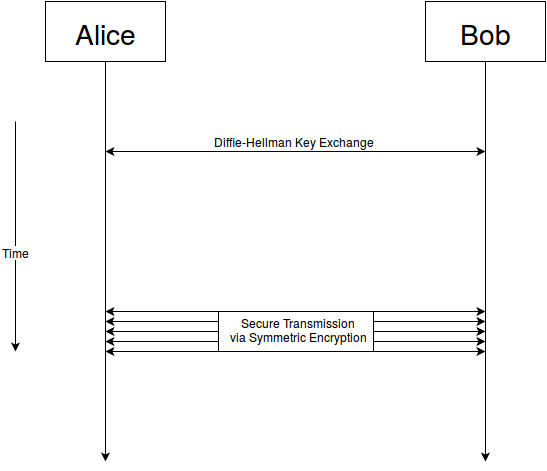
\includegraphics[width=0.8\textwidth]{pictures/archi}
	\vspace{0.5cm}
	\caption{Architecture of the a Diffie-Hellman based chat system}
	\label{fig:archi}
\end{figure}

\begin{figure}[h]
	\centering
	\vspace{0.5cm}
	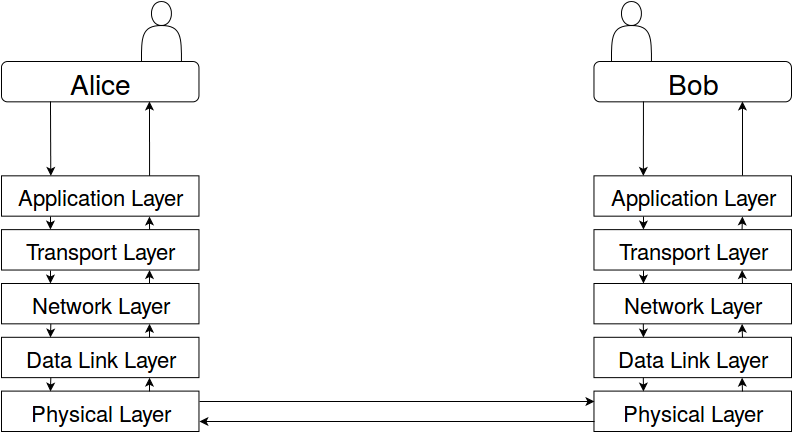
\includegraphics[width=0.7\textwidth]{pictures/tcpip}
	\vspace{0.5cm}
	\caption{Transmission of information over TCP/IP}
	\label{fig:tcpip}
\end{figure}

\newpage
Consider an active eavesdropper, say Mallory, who wants to eavesdrop upon the conversation of Alice and Bob. The eavesdropper can insert oneself between Alice and Bob before the key exchange occurs, and can actively transmit a different set of parameters (i.e. inject parameters) which the eavesdropper controls. This way, effectively two different conversations are created. One between Alice and Mallory, and the other between Mallory and Bob, as shown in Fig.~\ref{fig:mallory}. It is now upto Mallory to transmit messages correctly, or modify them, as per requirement. This may also lead up to further attacks which are outside the scope of this report.

\begin{figure}[h]
	\centering
	\vspace{0.5cm}
	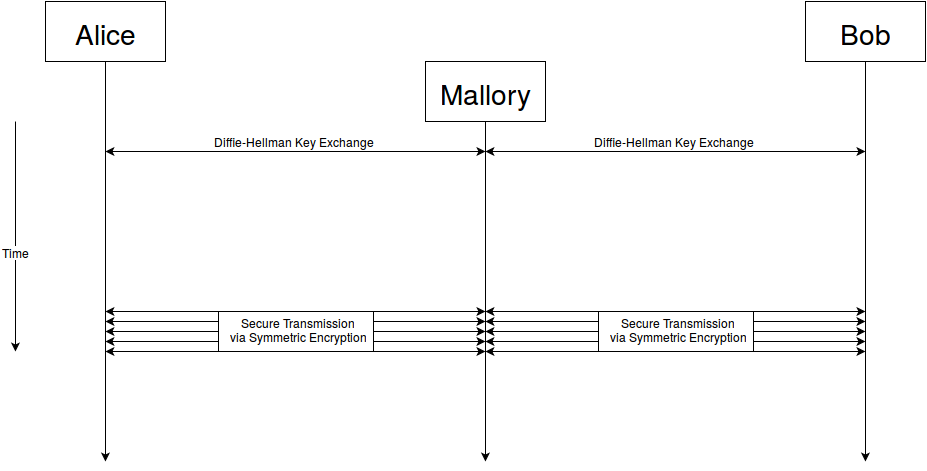
\includegraphics[width=0.8\textwidth]{pictures/mitm-mallory}
	\vspace{0.5cm}
	\caption{Active eavesdropping attack on Diffie-Hellman based chat system}
	\label{fig:mallory}
\end{figure}

\section{Algorithms Involved}
\label{sec:algo}

\begin{wrapfigure}{r}{0.4\textwidth}
	\centering
	\vspace{0.5cm}
	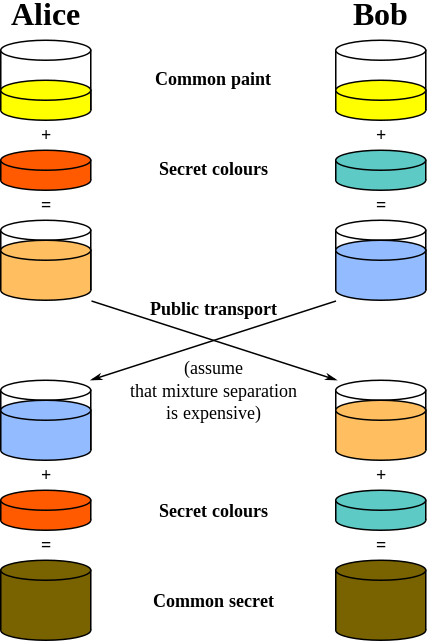
\includegraphics[width=0.3\textwidth]{pictures/paint}
	\vspace{0.5cm}
	\caption{Conceptual understanding of Diffie-Hellman key exchange protocol}
	\label{fig:paint}
\end{wrapfigure}

The Diffie-Hellman algorithm must be understood conceptually before actually looking at the algorithm. For this, Fig.~\ref{fig:paint} demonstrates this using the idea of mixing paint. The process begins by having the two parties, Alice and Bob, agree on an arbitrary starting color that does not need to be kept secret; in this example the color is yellow. Each of them selects a secret color–red and aqua respectively–that they keep to themselves. The crucial part of the process is that Alice and Bob now mix their secret color together with their mutually shared color, resulting in orange and blue mixtures respectively, then publicly exchange the two mixed colors. Finally, each of the two mix together the color they received from the partner with their own private color. The result is a final color mixture (brown) that is identical with the partner's color mixture.

If another party had been listening in on the exchange, it is computationally difficult for that person to determine the common secret color; in fact, when using large numbers rather than colors, this action is impossible for modern supercomputers to do in a reasonable amount of time.

\begin{figure}[h]
	\vspace{0.5cm}
	\begin{enumerate}
	\itemsep0em 
	\item 	\begin{tabbing} Alice \= and Bob, in public, agree on a $g$ and $p$, where \\
	\>$p$ is a cryptographically large prime, and\\
	\>$g$ is a primitive root modulo $p$.
		\end{tabbing}
	\item Alice chooses a secret integer $a$, and sends Bob $A = g^a \bmod p$.
	\item Bob chooses a secret integer $b$, and sends Alice $B = g^b \bmod p$.
	\item Alice calculates $s = B^a \bmod p$.
	\item Bob calculates $s = A^b \bmod p$.
	\item Alice and Bob now share common secret $s$.
	\end{enumerate}
	\caption{Diffie-Hellman Algorithm}
	\label{fig:dh-algo}
\end{figure}

Fig.~\ref{fig:dh-algo} describes the Diffie-Hellman Algorithm. Using this algorithm, Alice and Bob derive a common shared secret integer $s$. Using a cryptographic hashing function, it can be made into a cryptographic key which can be used for symmetric encryption. In the project described in this report, we have used the SHA256~\cite{sha} hash function to generate a 128 bit key, and 128 bit IV which is then used by the symmetric encryption algorithm AES128~\cite{aes} (in CBC mode) in order to communicate securely.

Fig.~\ref{fig:key-derivation} demonstrates an example key derivation algorithm which might be used further in the symmetric encryption. The shared secret $s$ is represented as a string, which is then hashed using SHA256. This 256 bit hashed value is then split midway to generate a 128 bit Key and 128 bit IV.

\begin{figure}[h]
	\centering
	\vspace{0.5cm}
	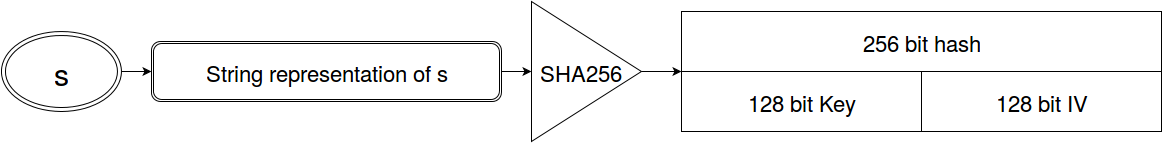
\includegraphics[width=0.9\textwidth]{pictures/key-derivation}
	\vspace{0.5cm}
	\caption{Key Derivation Algorithm}
	\label{fig:key-derivation}
\end{figure}

The MITM attacker uses the above mentioned concepts in order to form 2 connections as described in Section~\ref{sec:archi-n-working}.

\section{Implementation Details}
\label{sec:implementation}

% implementation detail on tools used and snaps

As mentioned in Section~\ref{sec:intro}, the project has been implemented in Python. The code will be made open-source after the publication of this report at \verb|https://github.com/jaybosamiya/DiffieHellman-ManInTheMiddle|. The code will be released under the MIT License.

AES128 CBC was implemented from scratch using AES128 ECB as a black box library. Cryptographically large primes were generated using PyCrypto, and Diffie-Hellman was implemented from scratch. Tkinter was used to design and implement the GUI. Network based interaction was implemented using the pwntools library.

The code is divided into multiple modules, each interacting with minimal coupling and strong coherence to provide highly re-usable code. The \verb|network| module handles network connections over TCP/IP. The \verb|gui| module takes care of interaction with the user. Fig.~\ref{fig:screenshots} shows some screenshots of the project in action. Diffie-Hellman shared secret derivation protocol is implemented in the \verb|diffie_hellman| module. The \verb|crypto_protocol| has the key derivation from the shared secret, and also handles the encryption and decryption of messages.

~

\noindent
The following describes the usage strings of the various parts of the project:
\begin{verbatim}
	    Server: run.py port_number
	    Client: run.py ip_address port_number
	    MITM  : mitm.py server_ip server_port client_port
\end{verbatim}

\begin{figure}[h]
	\centering
	\vspace{0.5cm}
	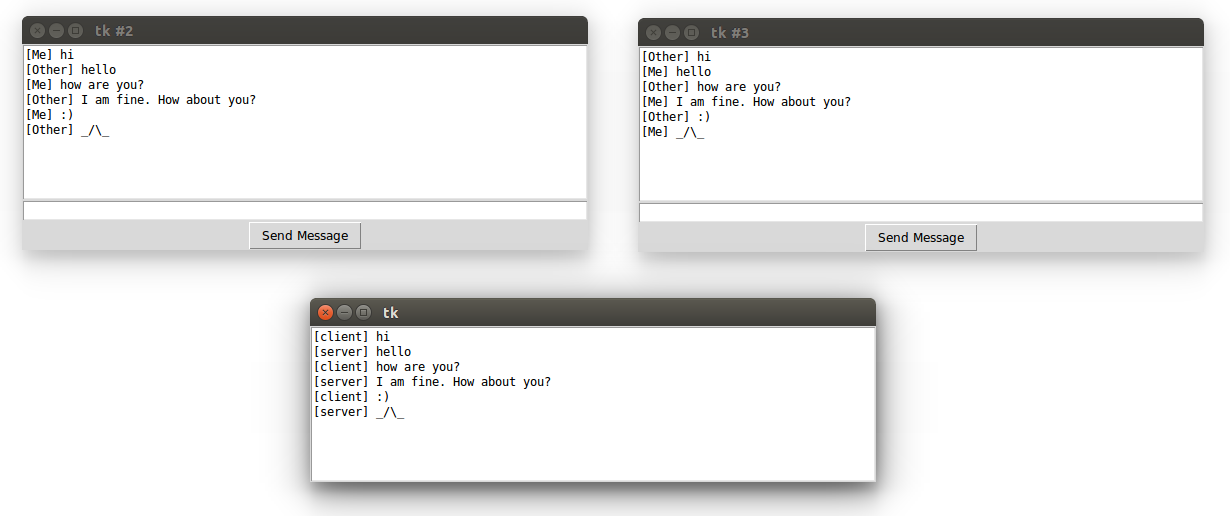
\includegraphics[width=0.9\textwidth]{pictures/screenshot}
	\vspace{0.5cm}
	\caption{Screenshots of the project}
	\label{fig:screenshots}
\end{figure}

\section{Novel Points of Work}
\label{sec:novel}

As far as we know, there is no other simulation of Diffie-Hellman along with the MITM attack which is both easy to demonstrate, as well as easy to understand. By writing a simple GUI and abstracting away most of the unnecessary interaction, our project demonstrates the problem of MITM. Also, through clean code written in easy to understand Python, it becomes easy to check through the code manually and understand exactly what is happening.

Our code is also highly reusable, and most parts of it can be re-used in various different projects, and simulations. It is also extremely good for prototyping different MITM attacks, some of which might be difficult to implement otherwise.

Also, this project presents a platform to learn ways to mitigate such attacks. It is designed in a way that it should not be hard to implement counter-measures to make such MITM attacks not usable anymore. Techniques for mitigating attacks are discussed in Section~\ref{sec:results}.

\section{Results}
\label{sec:results}

Through the design of the MITM attack, the security of the messages transferred is severely compromised. While in this project, the messages sent are only intercepted and displayed by the attacker, it is trivial to add functionality which allows the attacker to inject whatever data he/she wants to send.

All this mayhem is caused purely by the lack of authentication. The initial messages which have $p$, $g$, $A$, and $B$ are trusted without any indication of where they are actually from. This is a gross mistake on the part of the implementation.

Any message that is transmitted must be authenticated. This is one of the fundamental guidelines which is part of Cryptography. However, this rule is flouted often enough for such attacks to actually be practically possible.

One can easily use authenticated protocols for authentication. One such technique is the use of signing of whatever data is sent. For this, public-key cryptography might be used. This can be implemented into the project through the use of PGP~\cite{pgp} signing. An alternative is to use HMAC~\cite{hmac}, which would actually be preferable in the project as described in this report.

Also, the current MITM attack is possible through a cloaking of identity. If there exist a technique to authenticate the identity through another channel, then this attack is mitigated.

One other technique is to use an asymmetric cryptosystem, such as RSA~\cite{rsa}, to transmit a secret key from one person to another, and then use asymmetric cipher in order to maintain speed. 

\section{Comparison with Similar Works}
\label{sec:similar}

As described in Section~\ref{sec:novel}, there exist no similar works. However, there exist pre-existing implementation of AES128 CBC mode, with which we compared our encryption and decryption outputs, and they were found to be same. This goes on to prove that our implementation of AES128 CBC is correct. Also, through other implementations of Diffie-Hellman, we compared our outputs and they matched up when the same parameters were used. This further cements our confidence in the correctness of implementation. Since the project is only meant to be a simulation, an actual comparison of speeds with commercial products was not done, however, due to the tightness of the program loops, along with the minimal network transfer that is done, we are sure that the our project lies within only a small factor of speed of the fastest implementations of these algorithms.

\section{Conclusions}
\label{sec:conclusion}

Diffie-Hellman key exchange protocol was understood and implemented. Also, through the implementation of the MITM attack, various ways to break key exchange protocols were understood. Also, countermeasures against these were understood.

It was found that unauthenticated key exchange protocols are severely broken and should be phased out of usage. In their place, authenticated protocols must be used. Authenticated protocols verify the identity of the sender and/or receiver and thereby prevent the insertion of an active eavesdropper in the middle of the communication.

Also through the usage of asymmetric encryption, one can exchange keys. However, if done wrong, then even this suffers the same problem as other key exchange techniques.

\section{Future Work}
\label{sec:future}

By open-sourcing our project, we allow for further improvement of the simulation to show other techniques, and their problems. A strong direction to work in next would be in order to create some kind of attacker which also modifies messages going through it. This will allow for analysis of even more attacks. Also, simulation of various countermeasures for the attacks can be implemented and demonstrated, though this might be more difficult since demonstration of strength of a system is many times more difficult than demonstrating weakness.

\newpage

\bibliographystyle{plain}
\bibliography{bib}

\end{document}      

% https://www.owasp.org/index.php/Category:Cryptographic_Vulnerability